\chapter{Trabalhos futuros} \label{sec:atividades_futuras}
Como trabalhos futuros, ressalta-se a necessidade de  disponibilizar a ferramenta nas lojas de aplicativos Play Store e App Store, pois aumentaria o potencial de disseminação e adesão. É importante destacar que o setor de educação tem altas taxas de \textit{download} em ambas as lojas (Figura \ref{fig:statista}). Dessa maneira, seria possível criar uma base de usuários sólida e recorrente ao gerar valor para o público alvo. Além disso, eles receberiam atualizações de futuras mudanças e correções de problemas.

\begin{figure}[H]
\centering
    \caption{Categorias mais populares: App Store e Play Store}
    \label{fig:statista}
    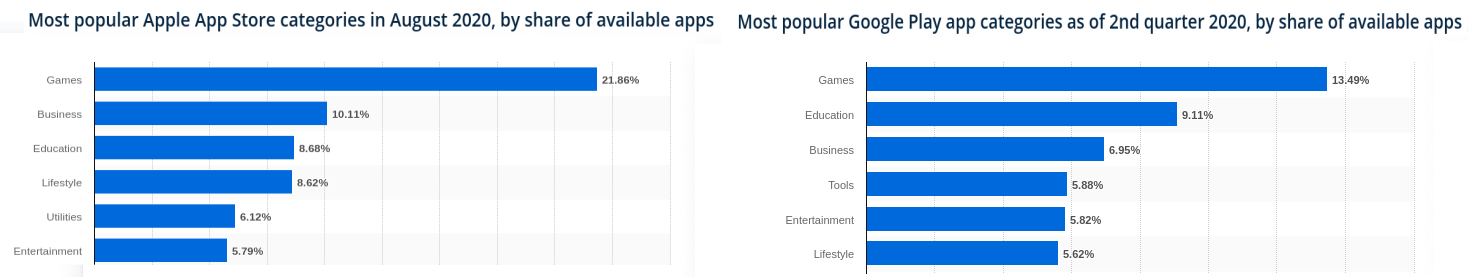
\includegraphics[width=1\textwidth]{Figuras/statista.png}
    
    Fonte: \href{https://www.statista.com/statistics/270291/popular-categories-in-the-app-store/}{App Store};  \href{https://www.statista.com/statistics/279286/google-play-android-app-categories/}{Play Store}
\end{figure}

Pretende-se ainda, construir uma plataforma de gestão para os professores. Nela, eles poderiam criar, editar e apagar disciplinas e aulas com conteúdos em texto, áudio e vídeo. Além disso, um dos objetivos é integrar o algoritmo de criação de palavras cruzadas à plataforma, a fim de facilitar sua construção e inserção no banco de dados para acesso pelos usuários por meio do aplicativo.

Falar aqui sobre a colaboração e inserção na tese de doutorado da Camila.

% No período de julho/2020 a novembro/2020, dando continuidade ao presente trabalho de iniciação científica, o bolsista dará ênfase às seguintes atividades:

% \begin{itemize}
    
%     %\item \textbf{Definição de requisitos da \crossword}: esta atividade consiste na elicitação dos requisitos da aplicação educacional móvel a ser desenvolvida.
%     \item \textbf{Projeto e Desenvolvimento da \crossword}: esta atividade consiste na continuidade da implementação da aplicação móvel.
%     \item \textbf{Avaliação da \crossword}: esta atividade consiste na condução de estudos  para avaliar a aplicação móvel desenvolvida. As avaliações devem considerar os aspectos pedagógicos e de usabilidade e acessibilidade da aplicação.
%     \item \textbf{Elaboração de artigos e relatórios}: esta atividade consiste em registrar as etapas conduzidas durante o desenvolvimento do trabalho e os resultados obtidos a partir dessa experiência. Os artigos desenvolvidos serão submetidos a congressos de iniciação científica e outros congressos nas áreas de interesse.
%     Nesse sentido, ressalta-se que as atividades conduzidas até o momento foram sintetizadas em um artigo completo, submetido ao 6º Congresso de Graduação da USP. 
% \end{itemize}

% \begin{table}[!ht]
% \centering
% \caption{\textit{Cronograma de atividades}}
% \label{tab:cronograma}
% \begin{tabular}{|l|c|c|c|c|c|c|c|c|c|c|c|c|}
% \hline
% \multirow{2}{*}{\textbf{Atividades}} & \multicolumn{12}{c|}{\textbf{Meses}} \\ \cline{2-13} 
%  & 1 & 2 & 3 & 4 & 5 & 6 & 7 & 8 & 9 & 10 & 11 & 12 \\ \hline
% 1) Conceitos - usabilidade e acessibilidade & $\checkmark$ & $\checkmark$ &  &  &  &  &  &  &  &  &  &  \\ \hline
% 2) Conceitos - aprendizagem móvel & $\checkmark$ & $\checkmark$ &  &  &  &  &  &  &  &  &  &  \\ \hline
% 3) Conceitos - ensino idosos & $\checkmark$ & $\checkmark$ &  &  &  &  &  &  &  &  &  &  \\ \hline
% 4) Artefatos &  & $\checkmark$ & $\checkmark$ & $\checkmark$ &  &  &  &  &  &  &  &  \\ \hline
% 5) Requisitos &  &  & $\checkmark$ & $\checkmark$ & $\checkmark$ &  &  &  &  &  &  &  \\ \hline
% 6) Projeto/MVP &  &  &  & $\checkmark$ & $\checkmark$ & $\checkmark$ &  &  &  &  &  &  \\ \hline
% 7) Levantamento e estudo de tecnologias &  &  &  &  & $\checkmark$ & $\checkmark$ &  &  &  &  &  &  \\ \hline
% 8) Desenvolvimento &  &  &  &  & $\checkmark$ & $\checkmark$ & $\checkmark$ & $\checkmark$ & $\checkmark$ & $\bullet$ &  &  \\ \hline
% 9) Avaliação &  &  &  &  &  &  &  &  &  & $\bullet$ & $\bullet$ & $\bullet$ \\ \hline
% 10) Artigos e relatórios &  &  &  &  &  & $\checkmark$ &  &  & $\checkmark$ &  &  & $\bullet$ \\ \hline
% \end{tabular}
% \end{table}

